Two families: symmetric cryptosystems use the same key for encryption and decryption. They rely on the principles from classical systems: substitution, permutation, and transposition. The reversing operation is dependent on the key.
Asymmetric cryptosystems, on the other hand, use a pair of mathematically related keys—one for encryption (public key) and another for decryption (private key)—relying on complex mathematical problems for security.

\subsection{Block Ciphers}
\begin{defn}
A \textbf{block cipher} is a deterministic cryptographic algorithm that operates on fixed-size blocks of data, typically \( n \) bits, using a symmetric key to perform encryption or decryption. It transforms a plaintext block of size \( n \) bits into a ciphertext block of the same size through a series of reversible, structured operations, and vice versa.

\end{defn}
\begin{figure}[h!]
    \centering
    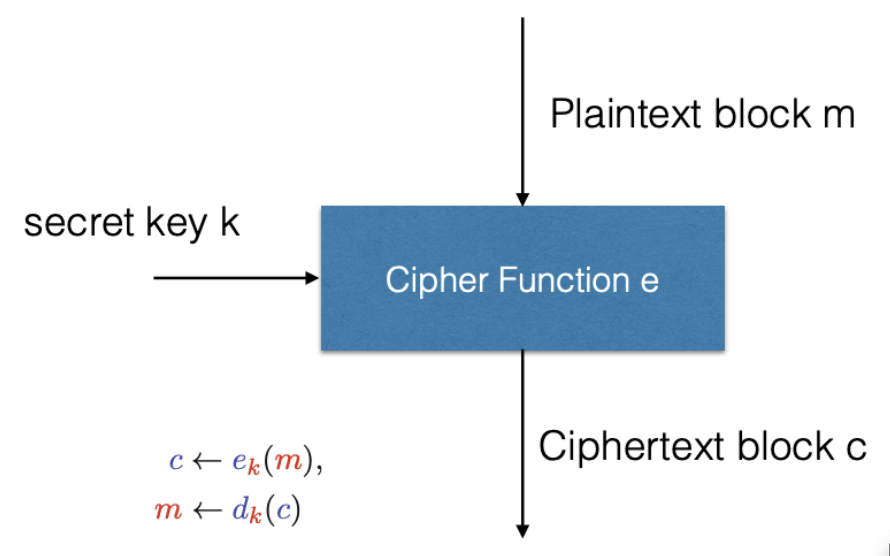
\includegraphics[width=0.5\textwidth]{img/blockcipher.png}
    \caption{Block Cipher}
    \label{fig:block_cipher}
\end{figure}

where
\begin{itemize}
    \item $m \in \{0,1\}^n$ is the plaintext block,
    \item $k \in K$ is the secret key, chosen from key space K,
    \item $e$ is the encryption function,
    \item $d$ is the decryption function,
    \item $c \in \{0,1\}^b$ is the ciphertext block.
\end{itemize}

NOTE: Block ciphers are not proper encryption schemes. You need to combine them with modes of operation! Otherwise your system will not be secure.

\subsubsection{Properties of Block Ciphers}
\begin{enumerate}
    \item Input Data Block: Plaintext is divided into equal-sized blocks.
    \item Encryption/Decryption: Each block undergoes multiple transformations (substitution, permutation, and mixing) to produce ciphertext.
    \item Key: A symmetric key is applied in multiple \emph{rounds} to ensure security.
    \item Padding: If the last block of plaintext is smaller than the block size, padding is added.
    \item Modes of Operation: Block ciphers work with data larger than one block by using modes like:
    \begin{itemize}
        \item ECB (Electronic Codebook)
        \item CBC (Cipher Block Chaining)
        \item GCM (Galois/Counter Mode)
    \end{itemize}
\end{enumerate}
Block ciphers are typically \emph{64 bits} (in DES), \emph{128 bits} (in AES) or more (in modern ciphers). They should act like a \emph{pseudorandom permutation} (PRP).

\begin{defn}
A \textbf{pseudorandom permutation} (PRP) is a function that defines a bijective (one-to-one and onto) mapping between input and output spaces, such that it is computationally indistinguishable from a truly random permutation when the key is unknown. 
\end{defn}

In order to limit the advantage of the adversary, the key space is kept very large (e.g. $Adv \ 1/|K|$). A block cipher is a \emph{building block} for designing a cipher (a PRP). A block cipher with a \emph{Mode of Operation} is a cipher. The goal is to design an IND-CCA secure cipher.

\subsubsection{Design}
DES and AES are iterated block ciphers. They \emph{repeat a simple round function}. The round $r$ can be fixed or variable. The more rounds, the higher the security of the cipher.
\begin{itemize}
    \item In each round, a round key, derived from the key $k$, is used (by key scheduling algorithm) to process a block
    \item The round function should be \emph{invertible}; for decryption the round keys are used in reverse order
    \item In DES: the round is invertible but not the round function
    \item In AES: both the round and the round function are invertible
\end{itemize}

\begin{defn}
    The \textbf{confusion-diffusion} paradigm is a fundamental design principle for secure cryptographic systems, particularly block ciphers.
    \begin{itemize}
        \item \textbf{Confusion:} Confusion ensures that the relationship between the key and the ciphertext is highly complex, making it difficult for an attacker to infer the key, even if they have access to multiple plaintext-ciphertext pairs. Split the block into smaller blocks and apply a
        substitution on each block.
        \item \textbf{Diffusion:} Diffusion ensures that the influence of a single bit of plaintext (or key) spreads widely over the ciphertext, so that changes in input affect many output bits.  Mix permutations so that local change can effect the
        whole block.
    \end{itemize}
\end{defn} \label{def:confusion_diffusion}

\begin{defn}
    A \textbf{substitution-permutation network} (SPN) is a design model for block ciphers. It consists of a series of linked operations, including substitution, permutation, and key mixing. It is a direct implementation of defintion \ref{def:confusion_diffusion}. 
\end{defn}
See figure \ref{fig:spn} for a diagram of an SPN.
\Comment{watch video on this for extra notes}

% \begin{figure}[h!]
%     \centering
%     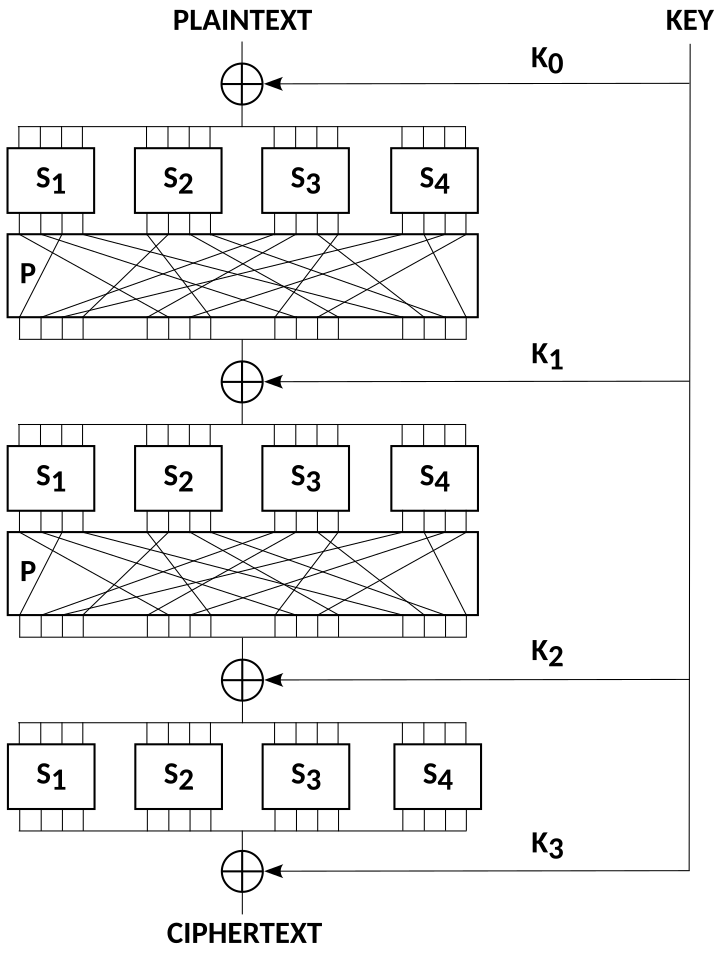
\includegraphics[scale=0.3]{img/spn.png}
%     \caption{A sketch of a substitution–permutation network with 3 rounds, encrypting a plaintext block of 16 bits into a ciphertext block of 16 bits. The S-boxes are the Si, the P-boxes are the same $P$, and the round keys are the $K_i$.}
%     \label{fig:spn}
% \end{figure}

\subsubsection{The Avalanche Effect}
A small change in the input must affect every bit of the output. This is called the \emph{avalanche effect}. It is a desirable property of block ciphers.
\begin{enumerate}
    \item The S-boxes (substitution box) are designed such that 1 bit effects at least 2 bits in the output of the boxes
    \item The mixing permutations are designed
\end{enumerate}

In principle, you need at least 7 rounds for a good diffusion. This is mathematically shown (outside of context for this course). Too few rounds (e.g. 1 or 2) will not provide security. The rounds can easily be reverted. 

\subsection{Feistel Ciphers}
\begin{defn}
A \textbf{Feistel cipher} is a symmetric structure used to construct block ciphers, including DES. It splits the plaintext block into two halves and performs a series of rounds of processing on the halves. Each round applies a function $F$ to one half and then combines it with the other half using a reversible operation, typically XOR.
\end{defn}

\begin{figure}[h!]
    \centering
    \begin{minipage}[t]{0.35\textwidth}
        \centering
        \vspace{0pt} % Ensure top alignment
        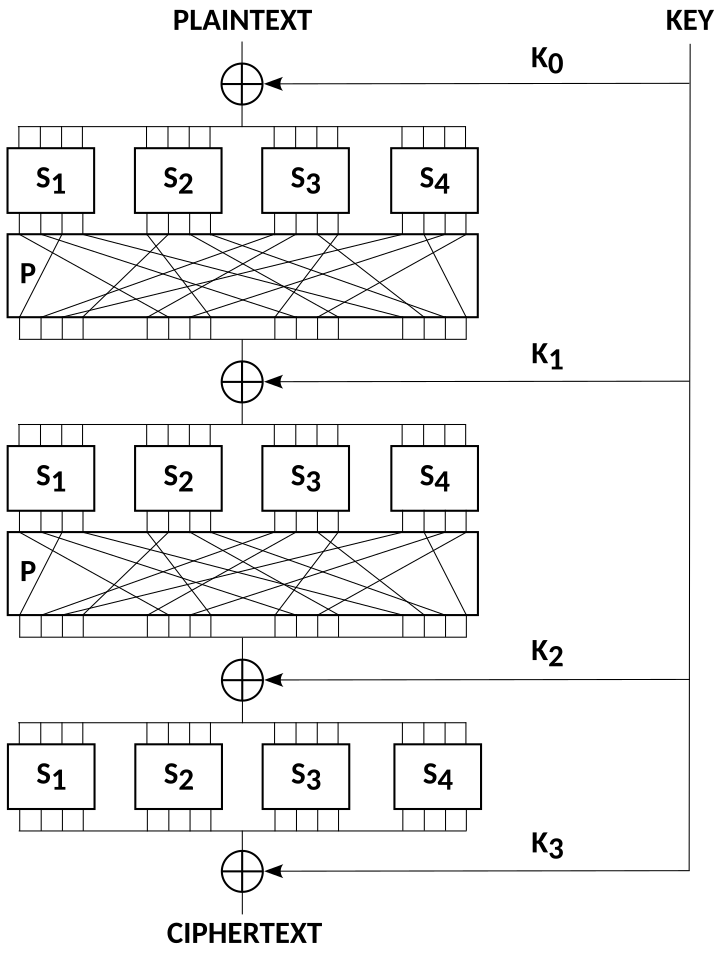
\includegraphics[width=\textwidth]{img/spn.png}
        \caption{A sketch of a substitution–permutation network with 3 rounds, encrypting a plaintext block of 16 bits into a ciphertext block of 16 bits. The S-boxes are the Si, the P-boxes are the same $P$, and the round keys are the $K_i$.}
        \label{fig:spn}
    \end{minipage}
    \hfill
    \begin{minipage}[t]{0.45\textwidth}
        \vspace{0pt} % Ensure top alignment
        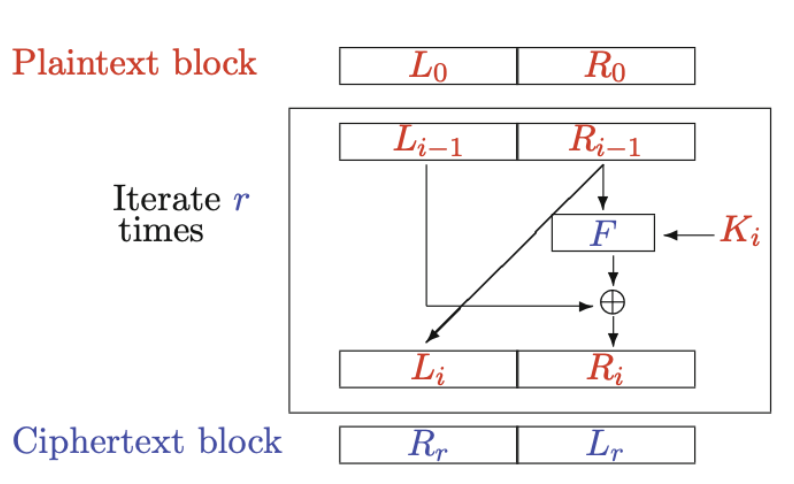
\includegraphics[width=\textwidth]{img/feistel.png}
        \caption{Basic operation of a Feistel cipher}
    \end{minipage}
\end{figure}

In a Feistel cipher, the round function is \emph{invertible}. It is different from an SPN, as that one is based on a non-invertible component. We can choose any function $F$ and still the round is invertible.
The same hardware/software can be used for encryption and decryption (just use the keys in reverse order). The security of the cipher depends on: the round keys, the number of rounds, and the function $F$.

\subsubsection{Encryption}
Given a plaintext block \( P \), a Feistel cipher processes it as follows:

\begin{enumerate}
    \item Initial split: Divide \( P \) into two equal-sized halves:
    \[
    P = (L_0, R_0)
    \]
    where \( L_0 \) and \( R_0 \) are the left and right halves, respectively.

    \item Rounds of encryption: For each round \( i \) (1 to \( n \)), compute:
    \[
    L_i = R_{i-1}
    \]
    \[
    R_i = L_{i-1} \oplus F(R_{i-1}, K_i)
    \]
    where:
    \begin{itemize}
        \item \( F \) is the round function (a non-linear function).
        \item \( K_i \) is the round key for round \( i \), derived from the main key.
    \end{itemize}

    \item Final Swap (Optional): After \( n \) rounds, the ciphertext \( C \) is obtained as:
    \[
    C = (R_n, L_n)
    \]
    (Note: The final swap is optional and does not affect decryption.)
\end{enumerate}

\subsubsection{Decryption}

The Feistel structure makes decryption straightforward because it is inherently reversible. Using the ciphertext \( C = (R_n, L_n) \):

\begin{enumerate}
    \item Initialize \( R_n \) and \( L_n \) as inputs.
    \item For each round \( i \) (in reverse order, from \( n \) to 1):
    \[
    R_{i-1} = L_i
    \]
    \[
    L_{i-1} = R_i \oplus F(L_i, K_i)
    \]
    \item Combine \( L_0 \) and \( R_0 \) to recover the original plaintext.
\end{enumerate}

The same function \( F \) and subkeys \( K_i \) are used in both encryption and decryption, but the subkeys are applied in reverse order during decryption.

\subsection{Data Encryption Standard (DES)}
DES is one of the earliest widely-used block ciphers. Not used anymore. But, still in ATMs (3DES). Key features are:

\begin{itemize}
    \item Block size: 64 bits
    \item Key length: 56 bits (with 8 parity bits)
    \item Number of rounds: 16
    \item 16 round keys, 48 bits each
    \item Structure: Feistel cipher
\end{itemize}

In the Feistel structure, each round splits the input into two halves: One half is directly passed to the next round. The other half is transformed using a combination of substitution, permutation, and the round key, then XORed with the other half.

\begin{figure}[h!]
    \centering
    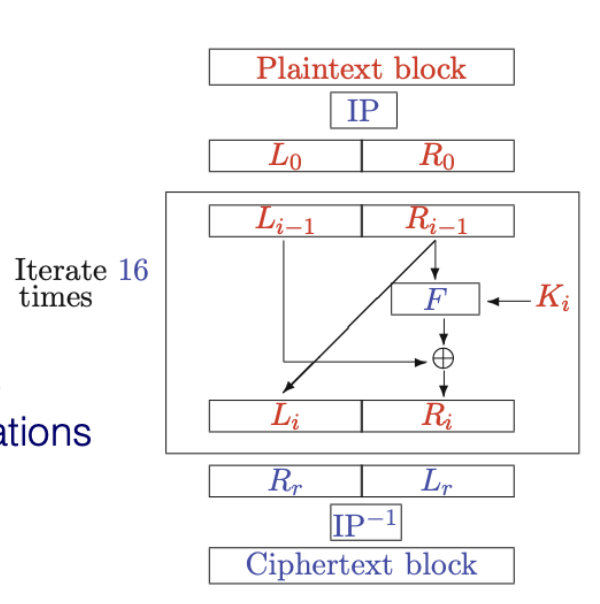
\includegraphics[width=0.35\textwidth]{img/des.png}
    \caption{DES as a Feistel structure}
    \label{fig:des}
\end{figure}

Operations:
\begin{itemize}
    \item 64 bits of plaintext block
    \item Perform an initial permutation (IP)
    \item Split the block into a left and right part
    \item Perform 16 rounds of \emph{identical operations}
    \item Join the half blocks together
    \item Perform a final reverse permutation (IP$^{-1}$)
\end{itemize}

\subsubsection{Function \texorpdfstring{$F$}{F}}

\subsubsection{S-boxes}

\subsubsection{P-box}

\subsubsection{Key Scheduling}

\subsubsection{Security of DES}
Weaknesses: 
\begin{itemize}
    \item The 56-bit key length is vulnerable to brute-force attacks. Modern computational power can crack DES in hours.
\end{itemize}

\subsection{Advanced Encryption Standard (AES)}

\subsection{Modes of Operation}